%\bibliographystyle{ieeetr}
%\bibliographystyle{splncs}
%\bibliographystyle{elsart-harv}
%\bibliographystyle{ipsjunsrt-e}
\bibliographystyle{ieicetr}




\Chapter{固有ベクトルで分類 --- グラフのスペクトルとデータのクラスタリング ---}


\Section{概要:グラフの解析によるデータの分類}


データを整理してグループにまとめることは基本的な解析のひとつである.
データクラスタリングの目標は,データの集合から
いくつかの自然なグループ(クラスタ)を見つけることである%
\footnote{クラスタは簡単に定義できるものではない.
クラスタ内のデータが互いに近く,%(内的結合(internal cohesion)),
クラスタが互いに離れている%(外的分離(external isolation))
という性質が望ましいとされるが,
データやクラスタ間の近い・遠い,似ている・似ていないことを
適切に測れるとは限らない.}.
様々な応用に対してクラスタリングの手法が
数多く提案されているが\cite{JainClusteringReview,JainClustering50years},
ここでは,クラスタリングのためのグラフ表現とその単純な固有値解析を紹介しよう.


\begin{figure}[hb]
\setlength{\unitlength}{1cm}
\begin{center}
%\fbox{
\begin{picture}(16,4.9)
\put(0,0.8){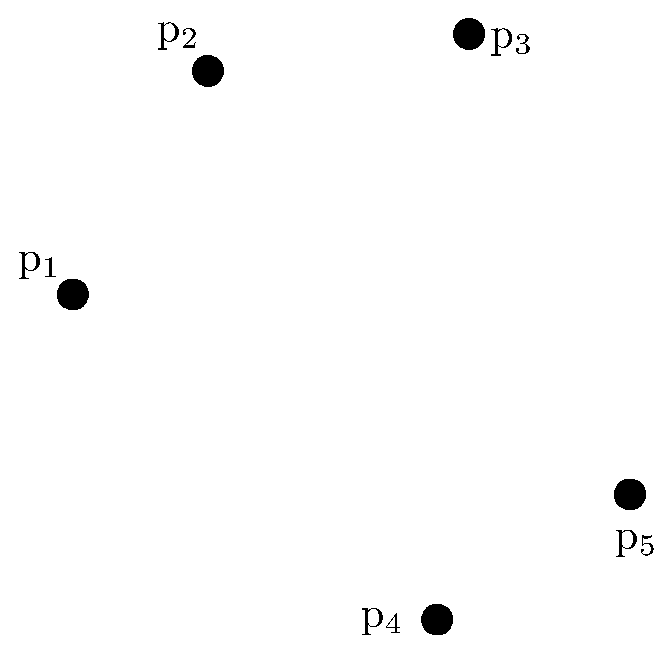
\includegraphics[width=4cm]{Ncut5points.eps}}
\put(6,0.8){\includegraphics[width=4cm]{Ncut5discon.eps}}
\put(12,0.8){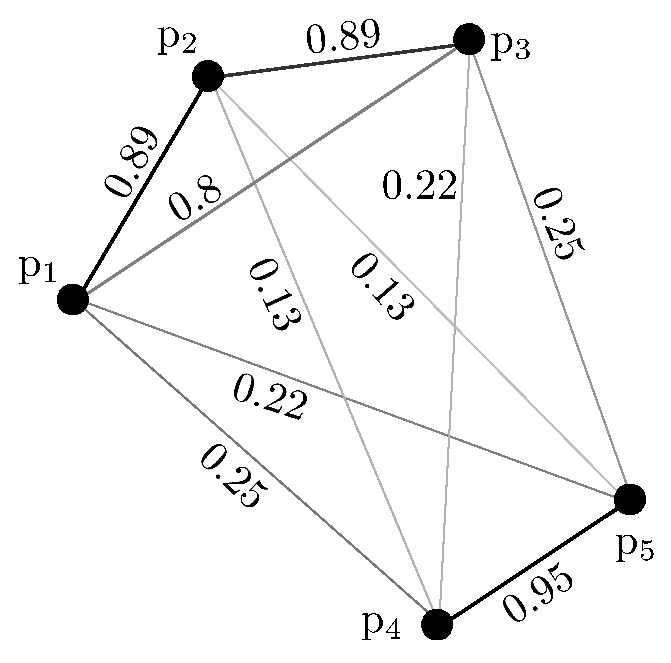
\includegraphics[width=4cm]{Ncut5simgra.eps}}
\put(2,0){(a)}
\put(8,0){(b)}
\put(14,0){(c)}
\end{picture}%}
 \caption{グラフの解析によるクラスタリング.グラフの節と枝はそれぞれ
データとデータ間の関係の深さを表す.
(a)与えられたデータ点.(b)クラスタを表す非連結グラフ.
(c)枝がデータ間の類似度を持っている類似度グラフ.}
\label{fig:Ncut5}
\end{center}
\end{figure}


データ集合が与えられたとき,
グラフを使って自動的にクラスタを見つけられるだろうか?
例えば,図\ref{fig:Ncut5}(a)のように,
5つのデータ点が与えられたときに2つのクラスタを見つけたいとする.
任意のデータ点の間のつながり(隣接)が分かっているならば,
図\ref{fig:Ncut5}(b)のようなグラフを作ることができる.
図の例では,他と連結していない2つのグラフの部分(連結成分)
によってグラフが構成されており,
2つのクラスタ$C_1=\{p_1,p_2,p_3\}$と$C_2=\{p_4,p_5\}$を特定できる.
このように,クラスタを表す連結成分を「計算」によって見つけることが,
グラフを用いたクラスタリングの目標である.

%How can we know the connectivity? % and compute the eigenvectors to obtain the clusters?
実際の応用では,データ間の隣接が明示的には与えられないかもしれないが,
データが持つ属性や特徴を使ってデータどうしの類似性か非類似性を
見積もれることがある(データ点の間の距離や内積など).
そのような場合は,例えば図\ref{fig:Ncut5}(c)のような
{\bf 類似度グラフ}(similarity graph)を作れる.
類似度グラフは,データ間の類似度を枝の重みとして与えた
単純グラフ\footnote{%
閉路も多重の枝も持たない無向グラフを単純グラフと呼ぶ.}である.
この類似度グラフの枝を切断して非連結のグラフにすることが
クラスタリングであると解釈できる.
その際,切断する枝の重みの和が最小になるように切断すべきである.




\Section{代数的なグラフの取り扱い}

\paragraph{隣接行列}
グラフを解析するため,{\bf 隣接行列}(adjacency matrix)を用いて
グラフを代数的に表すことができる.
$n$個の節を持つグラフ$G$の隣接行列$\mtr A$は,
節$i$から節$j$への枝の本数を第$i$行$j$列要素に持つ
$n\times n$行列である.
単純グラフは${0,1}$の2値の要素を持つ隣接行列で表される.
例えば,図\ref{fig:Ncut5}(b)の単純グラフの隣接行列は次のように書ける.
\begin{equation}
\mtr A=\smatrix{\normalsize}{ccccc}
{
0 & 1 & 1 & 0 & 0\\
1 & 0 & 1 & 0 & 0\\
1 & 1 & 0 & 0 & 0\\
0 & 0 & 0 & 0 & 1\\
0 & 0 & 0 & 1 & 0}
\end{equation}

\paragraph{次数行列}

節$i$から他の節への枝の本数を{\bf 次数}(degree)という.
隣接行列の第$i$行の行和は節$i$の次数に等しい.
$n$個の成分がすべて1のベクトルを$\vec 1_n$とすると,
$n$個の節の次数を成分に持つベクトルは
$\vec d=\mtr A\vec 1_n$のように計算できる.
次数を対角要素とする行列を{\bf 次数行列}(degree matrix)と定義する.
つまり,次数ベクトル$\vec d$を用いて$\mtr D=\diag(\vec d)$と書き表す.
図\ref{fig:Ncut5}(b)の単純グラフの次数ベクトルと次数行列は次のように書ける.
\begin{equation}
 \vec d=\mtr A\vec 1_n
=\smatrix{\small}{ccccc}
{
0 & 1 & 1 & 0 & 0\\
1 & 0 & 1 & 0 & 0\\
1 & 1 & 0 & 0 & 0\\
0 & 0 & 0 & 0 & 1\\
0 & 0 & 0 & 1 & 0}
\smatrix{\small}{c}{1\\ 1\\ 1\\ 1\\ 1}
=\smatrix{\small}{c}{2\\ 2\\ 2\\ 1\\ 1},
\quad \mbox{ }\quad
\mtr D=\diag\left(
\smatrix{\small}{c}{2\\ 2\\ 2\\ 1\\ 1}
\right)
=\smatrix{\small}{ccccc}
{
2 & 0 & 0 & 0 & 0\\
0 & 2 & 0 & 0 & 0\\
0 & 0 & 2 & 0 & 0\\
0 & 0 & 0 & 1 & 0\\
0 & 0 & 0 & 0 & 1}
\end{equation}


\paragraph{クラスタを表すベクトル}
$n$個のデータ点について,
成分がクラスタへの所属を表しているような$n$次元ベクトルを
{\bf クラスタ指示ベクトル}(cluster indicator)と呼ぶ.
図\ref{fig:Ncut5}のようなクラスタ$C_1=\{p_1,p_2,p_3\}$と$C_2=\{p_4,p_5\}$の
クラスタ指示ベクトルは,
それぞれ$\vec h^{(1)}=[1,1,1,0,0]$と$\vec h^{(2)}=[0,0,0,1,1]$である.

隣接行列$\mtr A$または次数行列$\mtr D$をクラスタ指示ベクトルに乗ずると,
クラスタに属す節の次数の総和が得られる.例えば,
\begin{equation}
\mtr A\vec h^{(1)}
=\smatrix{\small}{ccccc}
{
0 & 1 & 1 & 0 & 0\\
1 & 0 & 1 & 0 & 0\\
1 & 1 & 0 & 0 & 0\\
0 & 0 & 0 & 0 & 1\\
0 & 0 & 0 & 1 & 0}
\smatrix{\small}{c}{1\\ 1\\ 1\\ 0\\ 0}
=\smatrix{\small}{c}{2\\ 2\\ 2\\ 0\\ 0}
\quad \mbox{または}\quad
\mtr D\vec h^{(1)}
=\smatrix{\small}{ccccc}
{
2 & 0 & 0 & 0 & 0\\
0 & 2 & 0 & 0 & 0\\
0 & 0 & 2 & 0 & 0\\
0 & 0 & 0 & 1 & 0\\
0 & 0 & 0 & 0 & 1}
\smatrix{\small}{c}{1\\ 1\\ 1\\ 0\\ 0}
=\smatrix{\small}{c}{2\\ 2\\ 2\\ 0\\ 0}
\label{eq:counting degrees}
\end{equation}



\paragraph{ラプラシアン行列}
% variants
グラフ理論では,
グラフの{\bf ラプラシアン行列}(Laplacian matrix)が
$\mtr L=\mtr D-\mtr A$と定義されている.
{\bf ラプラシアン}とは,任意の点における値と
その近傍の平均値の差を測る2階微分演算子のことである.
もし,グラフの節を定義域として何らかの関数$f$が定義されていたら,
$\mtr L$はグラフ上で$f$のラプラシアンを計算する演算子になる.
例えば,図\ref{fig:Ncut5}(b)のグラフのラプラシアン行列$\mtr L$を
グラフ上の関数$f$に作用させると,
\begin{equation}
\mtr L
=\smatrix{\small}{ccccc}
{
2 & -1 & -1 & 0 & 0\\
-1 & 2 & -1 & 0 & 0\\
-1 & -1 & 2 & 0 & 0\\
0 & 0 & 0 & 1 & -1\\
0 & 0 & 0 & -1 & 1}
\quad \mbox{, }\quad
\mtr L\vec f=
\mtr L
\smatrix{\small}{c}{f(p_1)\\ f(p_2)\\ f(p_3)\\ f(p_4)\\ p(p_5)}
=
\smatrix{\scriptsize}{c}{
2\left(f(p_1)-\frac{f(p_2)+f(p_3)}{2}\right)\\
2\left(f(p_2)-\frac{f(p_1)+f(p_3)}{2}\right)\\
2\left(f(p_3)-\frac{f(p_1)+f(p_2)}{2}\right)\\
f(p_4)-f(p_5)\\
f(p_5)-f(p_4)}.
\end{equation}
という計算になる.
$\mtr L\vec f$の第1成分は,
$p_1$における$f$と,
隣接する$p_2$および$p_3$における$f$の平均値との
差になっていることがわかる.


ラプラシアン行列にはいくつかの興味深い性質がある.
\begin{itemize}
\item
任意のグラフについて
$\mtr L\vec 1_n=\mtr D\vec 1_n-\mtr A\vec 1_n=\vec d-\vec d=0\vec 1_n$が
必ず成り立つので,
$\mtr L$は少なくともひとつゼロの固有値を持ち,
その固有ベクトルは$\vec h=\vec 1_n$である.
\item
グラフが$k$個の連結成分からなるとき,
連結成分を表すクラスタ指示ベクトル$\vec h^{(l)}$ ($l=1,\dots,k$)が
ラプラシアン行列$\mtr L$のゼロの固有値に属する固有ベクトルになる.
このことは簡単に確認できる.
クラスタ$C_l$について,式(\ref{eq:counting degrees})のように
$\mtr A\vec h^{(l)}=\mtr D\vec h^{(l)}$が成り立つから,
$\mtr L\vec h^{(l)}=(\mtr D-\mtr A)\vec h^{(l)}=0\vec h^{(l)}$を得る.
\item
一般に,$\mtr L$のゼロの固有値が$k$個ならば,
グラフの連結成分は$k$個ある(演習問題\ref{ex:k indicators}).
\item
ラプラシアン行列の固有値は非負である(演習問題\ref{ex:L has nonnegative eigs}).
ラプラシアン行列$\mtr L$の固有値は{\bf グラフスペクトル}
(graph spectra)と呼ばれる.
\end{itemize}
ひとつの連結成分からなるグラフのラプラシアン行列はゼロの固有値をひとつ持つ.
グラフが複数の連結成分からなるかどうかは第2固有値から判明する.
それゆえ,第2固有値は{\bf 代数的連結度}(algebraic connectivity)と呼ばれる.
また,第2固有値に属する固有ベクトルは
{\bf Fiedlerベクトル}(Fiedler vector)\cite{Fiedler73}とも呼ばれる.



\Section{グラフのスペクトルと分割}

\paragraph{グラフの連結成分を見つける}
クラスタ指示ベクトルは,ラプラシアン行列のゼロの固有値に属する
固有ベクトルである.
この性質を利用して,グラフの連結成分として
クラスタを見つけるアルゴリズムを\ref{alg:finding disconnected components}に示す.
このように,データの関係を表現するグラフを記述する行列の
固有値解析によってクラスタを見つけることができる.


\begin{algorithm}[t]
\caption{連結成分を見つけるクラスタリング}
\label{alg:finding disconnected components}
\begin{algorithmic}[1]
\REQUIRE
隣接行列$\mtr A$;
\ENSURE クラスタの集合$\mathcal{C}=\{ C_1,\dots,C_k \}$;
\STATE
次数行列$\mtr D=\diag(\mtr A\vec 1_n)$を計算する;
\STATE
ラプラシアン行列$\mtr L=\mtr D-\mtr A$を計算する;
\STATE
$\mtr L$のゼロ固有値に属する固有ベクトル$\vec h^{(l)}$を計算する;
\STATE
$h_i^{(l)}\neq 0$ならば$i$を$C_l$に所属させる.
\end{algorithmic}
\end{algorithm}





\paragraph{類似度グラフを分割する}

%The clustering task can then be interpreted as cutting the similarity graph
%into disconnected components so as to minimize the sum of the cut-edge weights.


%\paragraph{Affinity matrix}
類似度グラフの枝のうち小さな類似度を持つものを切断して
クラスタを作ることを考える.
データ間の関係が類似度グラフとして与えられたとき,これを
{\bf 類似度行列}(affinity/similarity matrix)によって
代数的に表すことができる.
類似度行列は隣接行列を実数に拡張したようなものである.
類似度行列$\mtr W$の第$i$行$j$列要素は
節$i$から節$j$への枝の重み(つまり類似度)である.
図\ref{fig:Ncut5}(c)の類似度グラフの類似度行列は次のように書ける.
\begin{equation}
 \mtr W=
\smatrix{\small}{ccccc}
{
0 & 0.89 & 0.80 & 0.25 & 0.22\\
0.89 & 0 & 0.89 & 0.13 & 0.13\\
0.80 & 0.89 & 0 & 0.22 & 0.25\\
0.25 & 0.13 & 0.22 & 0 & 0.95\\
0.22 & 0.13 & 0.25 & 0.95 & 0}
\end{equation}
%
類似度グラフの次数行列$\mtr D$とラプラシアン行列$\mtr L$も
同様に類似度行列を用いて定義される.
\begin{equation}
 \mtr D=\diag(\mtr W\vec 1_n)
\end{equation}
\begin{equation}
 \mtr L=\mtr D-\mtr W
\end{equation}

類似度グラフのどの節も非ゼロの重みの枝をひとつ以上持つならば,
類似度グラフには非連結成分がない.
その類似度グラフのラプラシアン行列はひとつだけゼロ固有値を持ち,
固有ベクトルは$\vec h=\vec 1_n$である.
たとえ類似度グラフが明らかに$k$個の部分グラフからなっていても,
それらは小さな重みの枝で弱く結ばれているので,
アルゴリズム\ref{alg:finding disconnected components}によって
クラスタ指示ベクトル$\vec h^{(l)}$は得られない.
その代わり,類似度グラフのラプラシアン行列は$k$個の小さな固有値を持ち,
それらの固有ベクトルがクラスタを教えてくれる.
なぜならば,固有ベクトルがクラスタ指示ベクトルの近似になっているからである.
$\mtr W\vec h^{(l)}\neq\mtr D\vec h^{(l)}$なので,
$\mtr L\vec h^{(l)}=(\mtr D-\mtr W)\vec h^{(l)}\neq 0\vec h^{(l)}$である.
しかし,$\mtr D\vec h^{(l)}$と$\mtr W\vec h^{(l)}$の差は,
第$l$部分グラフの節と他の部分グラフの節の間の枝が持つ
小さな重みの総和を成分とする小さなベクトルに過ぎない.


図\ref{fig:Ncut5}(c)の類似度グラフの場合,
ラプラシアン行列の固有値は0, 0.99, 2.50, 2.96, 3.01である.
明らかに小さな固有値がふたつ存在し,
それらに属する固有ベクトルを列に並べると
\begin{equation}
 \mtr H_2=[\vec h^{(1)}, \vec h^{(2)}]=
\smatrix{\small}{rr}
{
0.45 & 0.33\\
0.45 & 0.43\\
0.45 & 0.33\\
0.45 & -0.55\\
0.45 & -0.55}.
\end{equation}
という行列を作れる.
固有ベクトル$\vec h^{(1)}$と$\vec h^{(2)}$はクラスタ指示ベクトルそのものではない.
しかし,行列$\mtr H_2$の全5行を2次元空間の5点のデータと見なしてプロットすると,
図\ref{fig:Ncut5clsind}のように2箇所に固まってクラスタが形成されていることがわかる.
これらのクラスタは$k$平均クラスタリング($k$-means clustering)や閾値処理程度の
簡単なベクトル量子化\footnote{%
小数点以下を四捨五入するなど,実数を何種類かの整数(または記号)のひとつに
置き換えることを量子化という.
同様に,ベクトルを何種類かの整数(または記号)のひとつに対応させることを
ベクトル量子化と呼ぶ.
ベクトルで表されるデータのクラスタリングはベクトル量子化の一手法である.
}で特定することができる.


\begin{figure}[h]
\setlength{\unitlength}{1cm}
\begin{center}
%\fbox{
\begin{picture}(6,5)
\put(0,0){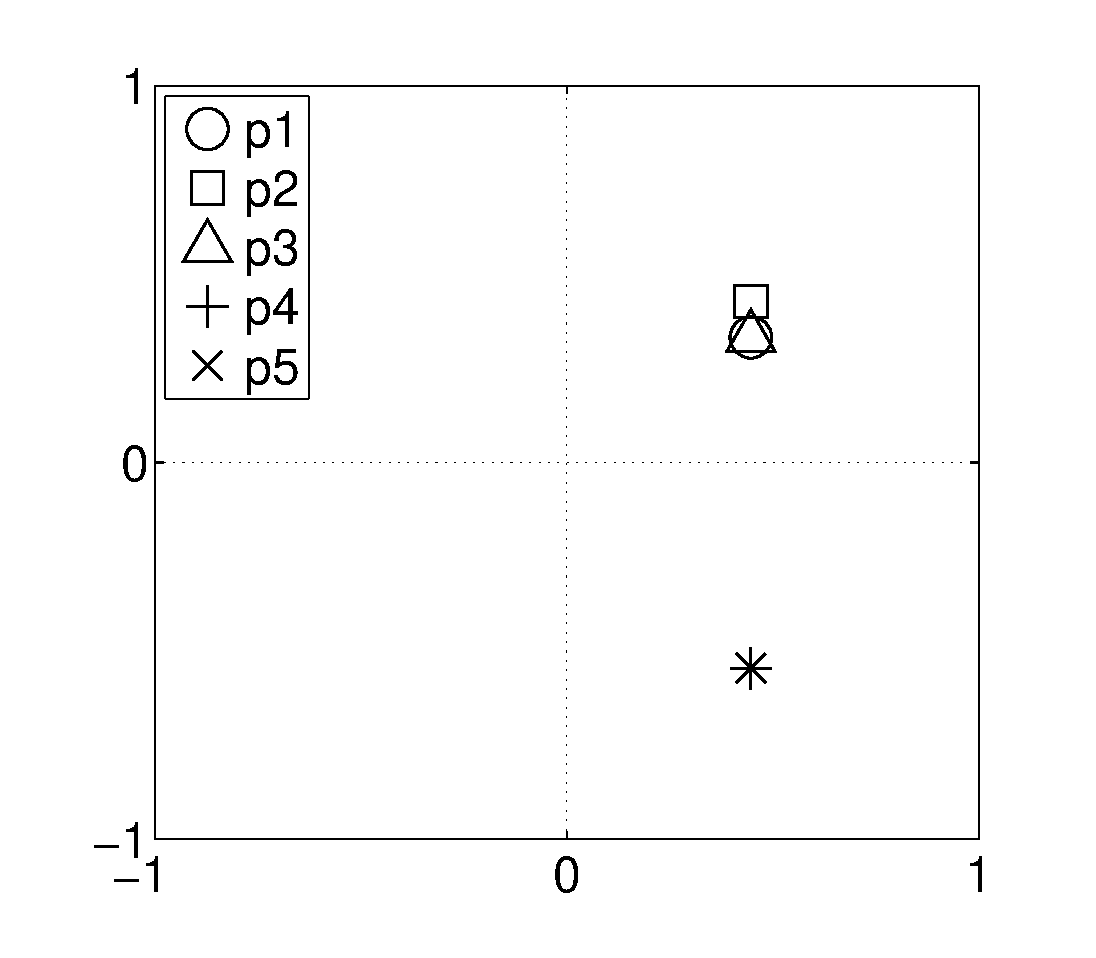
\includegraphics[width=6cm]{Ncut5clsind.eps}}
\end{picture}%}
 \caption{$\mtr H_2$の5行が2次元空間でふたつの密なクラスタを呈す.}
\label{fig:Ncut5clsind}
\end{center}
\end{figure}

このように,グラフを表す行列から固有ベクトルを計算すると,
類似度グラフの分割による$n$個のデータ点のクラスタリングは,
$k$次元空間の$n$個の点のクラスタリングに帰着する.


\Section{スペクトラルクラスタリングのアルゴリズム}

\begin{algorithm}[t]
\caption{スペクトラルクラスタリング}
\label{alg:spectral clustering}
\begin{algorithmic}[1]
\REQUIRE
類似度行列$\mtr W$, クラスタ数$k$;
\ENSURE クラスタの集合$\mathcal{C}=\{ C_1,\dots,C_k \}$;
\STATE
次数行列$\mtr D=\diag(\mtr W\vec 1_n)$を計算する;
\label{step:D}
\STATE
Rcut\cite{Hagen92}の場合: \\
ラプラシアン行列$\mtr L=\mtr D-\mtr W$の$k$個の小さな固有値に属する
固有ベクトルを列に並べた行列
$\mtr X_k=[\vec x^{(1)},\dots,\vec x^{(k)}]\in\mathbb{R}^{n\times k}$を作る;\\
Ncut\cite{Shi00,Yu03})の場合: \\
正規化類似度行列$\mtr S=\mtr D^{-1/2}\mtr W\mtr D^{-1/2}$の
$k$個の大きな固有値に属する
固有ベクトルを列に並べた行列
$\mtr X_k=[\vec x^{(1)},\dots,\vec x^{(k)}]\in\mathbb{R}^{n\times k}$を作る;
\label{step:eigen}
\STATE
$\mtr X_k$の各行ベクトルを正規化する;
\STATE
ベクトル量子化によって各データ点をクラスタのひとつ$C_l\in\mathcal{C}$に所属させる: 
典型的には,$\mtr X_k$の$n$本の行ベクトルに$k$平均クラスタリングを適用する.
\end{algorithmic}
\end{algorithm}

固有値解析に基づくデータクラスタリングを
アルゴリズム\ref{alg:spectral clustering}に示す.
このアルゴリズムは,グラフの$k$分割の「コスト」を最小化する問題について,
クラスタ指示ベクトルを離散2値から実数へ緩和することで導出される.
グラフを切断するコストは,クラスタの下記の性質を考慮して設計されている.
\begin{description}
\item[外的分離(external isolation)]
クラスタが互いに離れていること.
第$l$クラスタ$C_l$の全データ点と他のクラスタのデータ点をつなぐ枝の重みの和は,
${\vec h^{(l)}}^\top\mtr L\vec h^{(l)}$のように計算できる.この値は小さいほどよい.
$C_l$が他のクラスタから離れるほど小さくなるからである.
\item[内的結合(internal cohesion)]
クラスタ内のデータが互いに近いこと.
第$l$クラスタ$C_l$内のデータの個数は${\vec h^{(l)}}^\top\vec h^{(l)}$である.
$C_l$内のデータから他の節への枝の重みの総和は${\vec h^{(l)}}^\top\mtr D\vec h^{(l)}$
のように計算できる.
どのクラスタについても,これらの量が大きいほどよい.
各クラスタがよくまとまっていて,バランスがとれているほど大きくなるからである.
\end{description}

%There are some variants of spectral clustering.
スペクトラルクラスタリングのためのグラフ切断コストがいくつか設計されている.
\begin{eqnarray}
&\mbox{Ratio cut \cite{Hagen92}}:&
J\msub{Rcut}(\mtr H)=
\sum_{l=1}^k\frac{{\vec h^{(l)}}^\top\mtr L\vec h^{(l)}}{\vec {h^{(l)}}^\top\vec h^{(l)}}\label{eq:Rcut cost}\\
&\mbox{Normalized cut \cite{Shi00,Yu03}}:&
J\msub{Ncut}(\mtr H)=
\sum_{l=1}^k\frac{{\vec h^{(l)}}^\top\mtr L\vec h^{(l)}}{{\vec h^{(l)}}^\top\mtr D\vec h^{(l)}}\label{eq:Ncut cost}
%\\
%&\mbox{Min-max cut \cite{Shi00,Yu03}}:&
%J\msub{Mcut}(\mtr H)=
%\sum_{l=1}^k\frac{\vec h_l^\top\mtr L\vec h_l}{\vec h_l^\top\mtr W\vec h_l}
\end{eqnarray}
コスト$J\msub{Rcut}(\mtr H)$や$J\msub{Ncut}(\mtr H)$は,
$k$本のクラスタ指示ベクトル$\vec h^{(l)}$ ($l=1,\dots,k$)の関数である.
コストが最小になる$\mtr H=[\vec h^{(1)},\dots,\vec h^{(k)}]$を探す問題は
組合せ最適化問題である.
式(\ref{eq:Rcut cost})や式(\ref{eq:Ncut cost})を最小化する問題を
制約付き対角和最小問題に書き換え,
クラスタ指示ベクトル$\vec h^{(l)}$を
実ベクトル$\vec x^{(l)}\in\mathbb{R}^n$と見なすと近似的な解法が得られる.
実数のクラスタ指示ベクトル$\vec x^{(l)}$は次のような固有値問題の
固有ベクトルとして求まる.
\begin{eqnarray}
&\mbox{Ratio cut}:&
\mtr L\vec x^{(l)}=\lambda_l\vec x^{(l)}\\
&\mbox{Normalized cut}:&
\mtr S\vec x^{(l)}=\mu_l\vec x^{(l)}
%\mtr L\vec y_l=\lambda_l\mtr D\vec y_l,\quad \vec x_l=\mtr D^{1/2}\vec y_l\\
%&\mbox{Min-max cut}:&
\end{eqnarray}
ただし,$\lambda_l$ ($l=1,\dots,k$) は$\mtr L$の$k$個の小さな固有値,
$\mu_l$ ($l=1,\dots,k$) は$\mtr S=\mtr D^{-1/2}\mtr W\mtr D^{-1/2}$の
$k$個の大きな固有値である.
導出の詳細は文献\cite{Luxburg07}が詳しい.





\Section{演習問題}
\begin{enumerate}
\item
\label{ex:k indicators}
連結成分が$k$個あるグラフ$G$のラプラシアン行列を$\mtr L$とする.
$\mtr L$のゼロの固有値が$k$個ならば,$G$の連結成分は$k$個あることを証明せよ.\\
ヒント:
連結成分を表す$k$本のクラスタ指示ベクトル$\vec h^{(l)}$ ($l=1,\dots,k$)が
$\mtr L$の固有ベクトルであり,その固有値はゼロであることから,
$\mtr L$の固有値のうち少なくとも$k$個はゼロであると言える.
$\mtr L$のゼロの固有値に属する固有ベクトルは,
クラスタ指示ベクトルまたはその線形結合で表せるベクトルに
限られることを示せばよい.
\item
\label{ex:L has nonnegative eigs}
ラプラシアン行列の固有値は非負であることを証明せよ.\\
ヒント:
関数$q(\vec h)=\vec h^\top\mtr L\vec h$を,行列$\mtr L$の二次形式と呼ぶ.
$\|\vec h\|_2=1$の条件下で二次形式$q(\vec h)$の極値は$\mtr L$の固有値となる.
また,隣接行列$\mtr A$の要素を用いてラプラシアン行列$\mtr L=\mtr D-\mtr A$の
二次形式を書き表すと$q(\vec h)\geq 0$が示せる.
%ラプラシアン行列$\mtr L$は対称行列なので,固有ベクトルは互いに直交する.
%固有ベクトルを列に並べた行列を$\mtr H$とすると$\mtr H^\top=\mtr H$が成り立つ.
%$\mtr L=\mtr H\mtr{\mit\Lambda}\mtr H^\top$
%二次形式の
%対称行列の固有値
\item
スペクトラルクラスタリングを2次元の点集合
(例えば\href{http://cs.joensuu.fi/sipu/datasets/}{Clustering datasets\\ (http://cs.joensuu.fi/sipu/datasets/)}に適用せよ.
ただし,点$\vec p^{(i)}$と点$\vec p^{(j)}$ ($i\neq j$)の類似度$w_{ij}$を
次式のように定義する.
\begin{equation}
 w_{ij}=\exp\left(-\frac{\| \vec p^{(j)}-\vec p^{(i)} \|_2^2}{2\sigma^2}\right)
\end{equation}
$\sigma$は尺度のパラメタで,近いと見なす点間の距離の目安である.
例えば,下記のMATLABコードのようにデータ集合
\href{http://cs.joensuu.fi/sipu/datasets/spiral.txt}{Spiral}または
\href{http://cs.joensuu.fi/sipu/datasets/D31.txt}{D31}に試してみよ.
\lstset{language=Matlab}
\lstset{basicstyle={\tt},identifierstyle={\bfseries},keywordstyle={\bfseries}}
\lstset{tabsize=2,showstringspaces=false}
\lstset{commentstyle={\color[rgb]{0,0.5,0}}}
\lstset{flexiblecolumns=true}
\lstset{classoffset=1,breaklines=true,morecomment=[l]{//}}
%\lstset{columns=[l]{fullflexible}}
%\lstset{numbers=left,stepnumber=1,numberstyle={\scriptsize},numbersep=4ex}
\lstset{frame=tBlR,rulecolor={\color[gray]{0.75}},rulesepcolor={\color[gray]{0.75}}}
\lstset{framesep=2ex}
\lstset{xleftmargin=4ex,xrightmargin=4ex}
%\lstset{backgroundcolor={\color[rgb]{1,1,0.95}}}
\begin{lstlisting}
close all

% データ集合を読み込む.
data = load('spiral.txt');
n = size(data, 1);

% クラスタ数と尺度を設定する.
k = 3; sigma = 1.0;

% 類似度行列Wと正規化類似度行列Sを計算する.
pairdist = pdist(data(:,1:2));
W = exp(- squareform(pairdist.^2 / (2.0 * sigma.^2))) - eye(n, n);
Dinvsq = diag(1./sqrt(sum(W, 2)));
S = Dinvsq * W * Dinvsq;

% 固有ベクトルXと固有値Mを求める.
[X, M] = eig(S);
[M,idx] = sort(diag(M),'descend');
figure, plot(1:n, M)

% 上位k本の固有ベクトルを取り出して行を正規化する.
X = X(:, idx(1:k));
X = diag(1./sqrt(sum(X.^2, 2))) * X;

% k平均クラスタリングでベクトル量子化する.
c = kmeans(X, k, 'emptyaction', 'singleton');

% 結果を表示する.
marker10 = {'+', '*', 'x', '^', 'v', 's', 'p', '^', 'd', 'v'};
col = colormap(lines(16));
figure;
hold on
for t = 1:k,
    p = find(c == t);
    plot(data(p,1), data(p,2), marker10{mod(t,10)+1}, 'Color', col(mod(t,16)+1,:));
end
hold off
\end{lstlisting}
数千個のデータ点のクラスタリング
(数百万個以上の非ゼロ要素を持つ行列の固有ベクトル計算)
は数分かかるので注意せよ.


\item\yeeks
Webサイト
\href{http://www.cise.ufl.edu/research/sparse/matrices/}{the University of Florida Sparse Matrix Collection\\ (http://www.cise.ufl.edu/research/sparse/matrices/)}\\
を見て,
ひとつ行列を選べ
(例えば,{\tt c-45.mat}, {\tt jazz.mat}, {\tt wiki-Vote.mat}, {\tt netscience.mat}など).
その行列は無向グラフまたは2部グラフの類似度行列と見なせる.
スペクトラルクラスタリングを適用せよ.
固有値をプロットしてクラスタ数を推測せよ.
できればグラフのクラスタを可視化せよ.\\
ヒント:Ncutを適用するサンプルコードは下記のとおりである.
\begin{lstlisting}
close all
load('jazz.mat'); k = 4;
W = abs(Problem.A);
[m, n] = size(W);
Dinvsq1 = spdiags(1./sqrt(sum(W, 1)'), 0, n, n);
Dinvsq2 = spdiags(1./sqrt(sum(W, 2)), 0, m, m);
S = Dinvsq2 * W * Dinvsq1;

% スパース行列の特異値分解によって上位20*k個の固有値,固有ベクトルを計算する.
[X, M,~] = svds(S,20*k);
M = diag(M);
figure,plot(1:length(M), M, 'o')

X = X(:,1:k);
X = spdiags(1./sqrt(sum(X.^2, 2)), 0, m, m) * X;
c = kmeans(X, k, 'emptyaction', 'singleton');
\end{lstlisting}
\end{enumerate}





{\footnotesize
\bibliography{mybib_cls}
}



